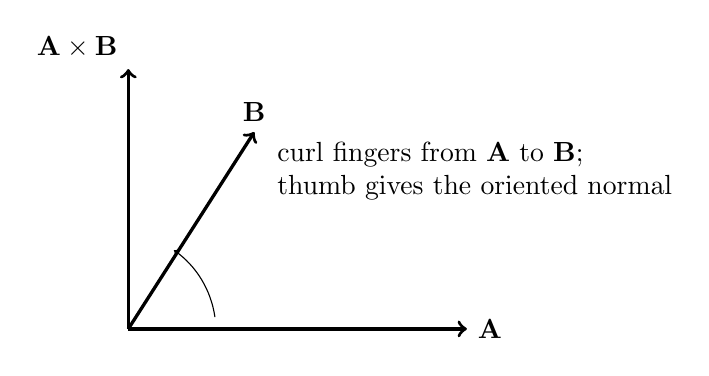
\begin{tikzpicture}[scale=1.0]
  \coordinate (O) at (0,0);
  \draw[->,very thick] (O)--(4.3,0) node[right] {$\mathbf A$};
  \draw[->,very thick] (O)--(1.6,2.5) node[above] {$\mathbf B$};
  \draw[->,very thick] (O)--(0,3.3) node[above left] {$\mathbf A\times\mathbf B$};
  \draw[->] (1.1,0.15) arc[start angle=8,end angle=55,radius=1.25];
  \node[align=left] at (4.4,2.0) {curl fingers from $\mathbf A$ to $\mathbf B$;\\thumb gives the oriented normal};
\end{tikzpicture}
